\EnableTitleSlide
\section{Aufbau \& Entwicklung \\ der Anwendung}

\begin{frame}{egg}
    \begin{columns}[c]
        \column{.7\textwidth}
            \begin{itemize}
                \item \textbf{egg}: \textbf{e}-\textbf{g}raphs \textbf{g}ood (\url{https://egraphs-good.github.io/})
                \item Bibliothek in Rust zur Erstellung von E-Graphs
                \item \textbf{Paper}: Willsey u.a. 2021~\cite{2021-egg} (\url{https://doi.org/10.1145/3434304})
            \end{itemize}\hspace{2.5cm}
        \column{.3\textwidth}
            
\includegraphics[scale=1.9]{utils/egg.pdf}
    \end{columns}
\end{frame}

\begin{frame}{Google Colab Notebook}
    \begin{columns}[c]
        \column{.7\textwidth}
            \begin{itemize}
                \item \textbf{Google Colab Notebook}
                \item Prototyp in Python basierend auf egg
                \item \textbf{Zachary DeVito}~\cite{devito} (\url{https://colab.research.google.com/drive/1tNOQijJqe5tw-Pk9iqd6HHb2abC5aRid?usp=sharing})
            \end{itemize}\hspace{-2.5cm}
        \column{.3\textwidth}
            
\includegraphics[scale=0.15]{utils/colab.png}
    \end{columns}
\end{frame}

\begin{frame}{Anwendung (1)}
    \begin{center}
        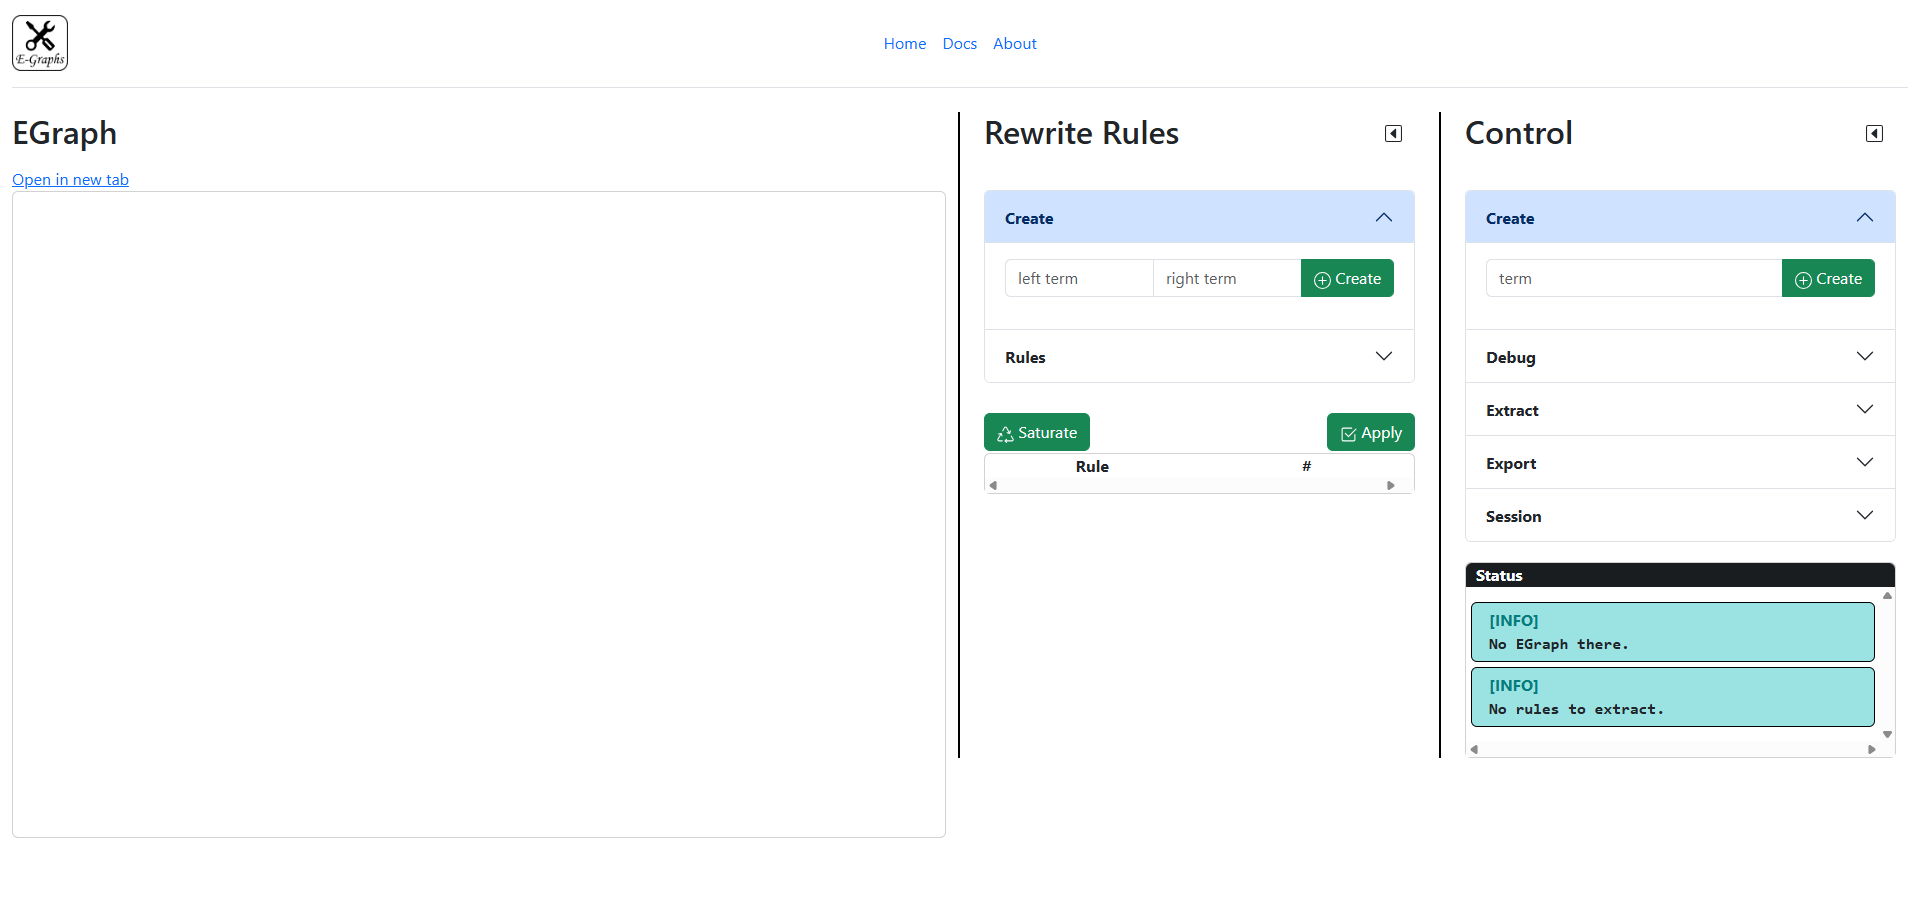
\includegraphics[scale=0.3]{utils/anwendung/anwendung1.png}
    \end{center}
\end{frame}

\begin{frame}{Anwendung (2)}
    \begin{center}
        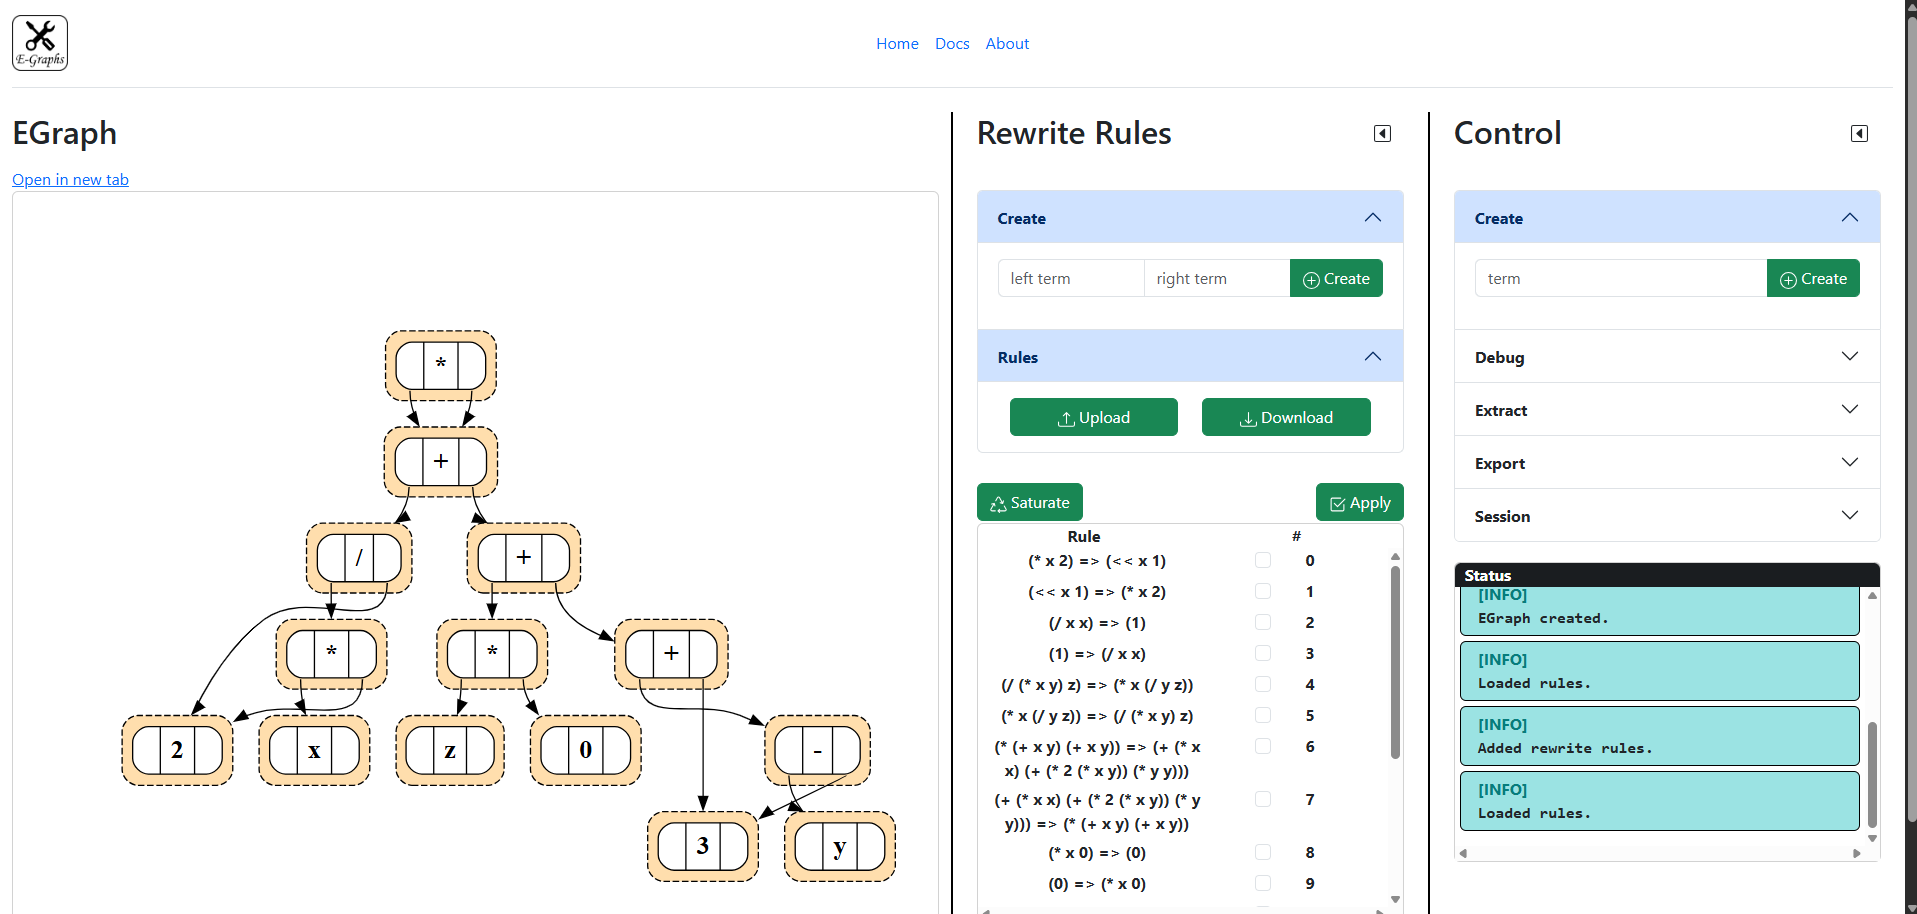
\includegraphics[scale=0.3]{utils/anwendung/anwendung2.png}
    \end{center}
\end{frame}

\begin{frame}{Anwendung (3)}
    \begin{center}
        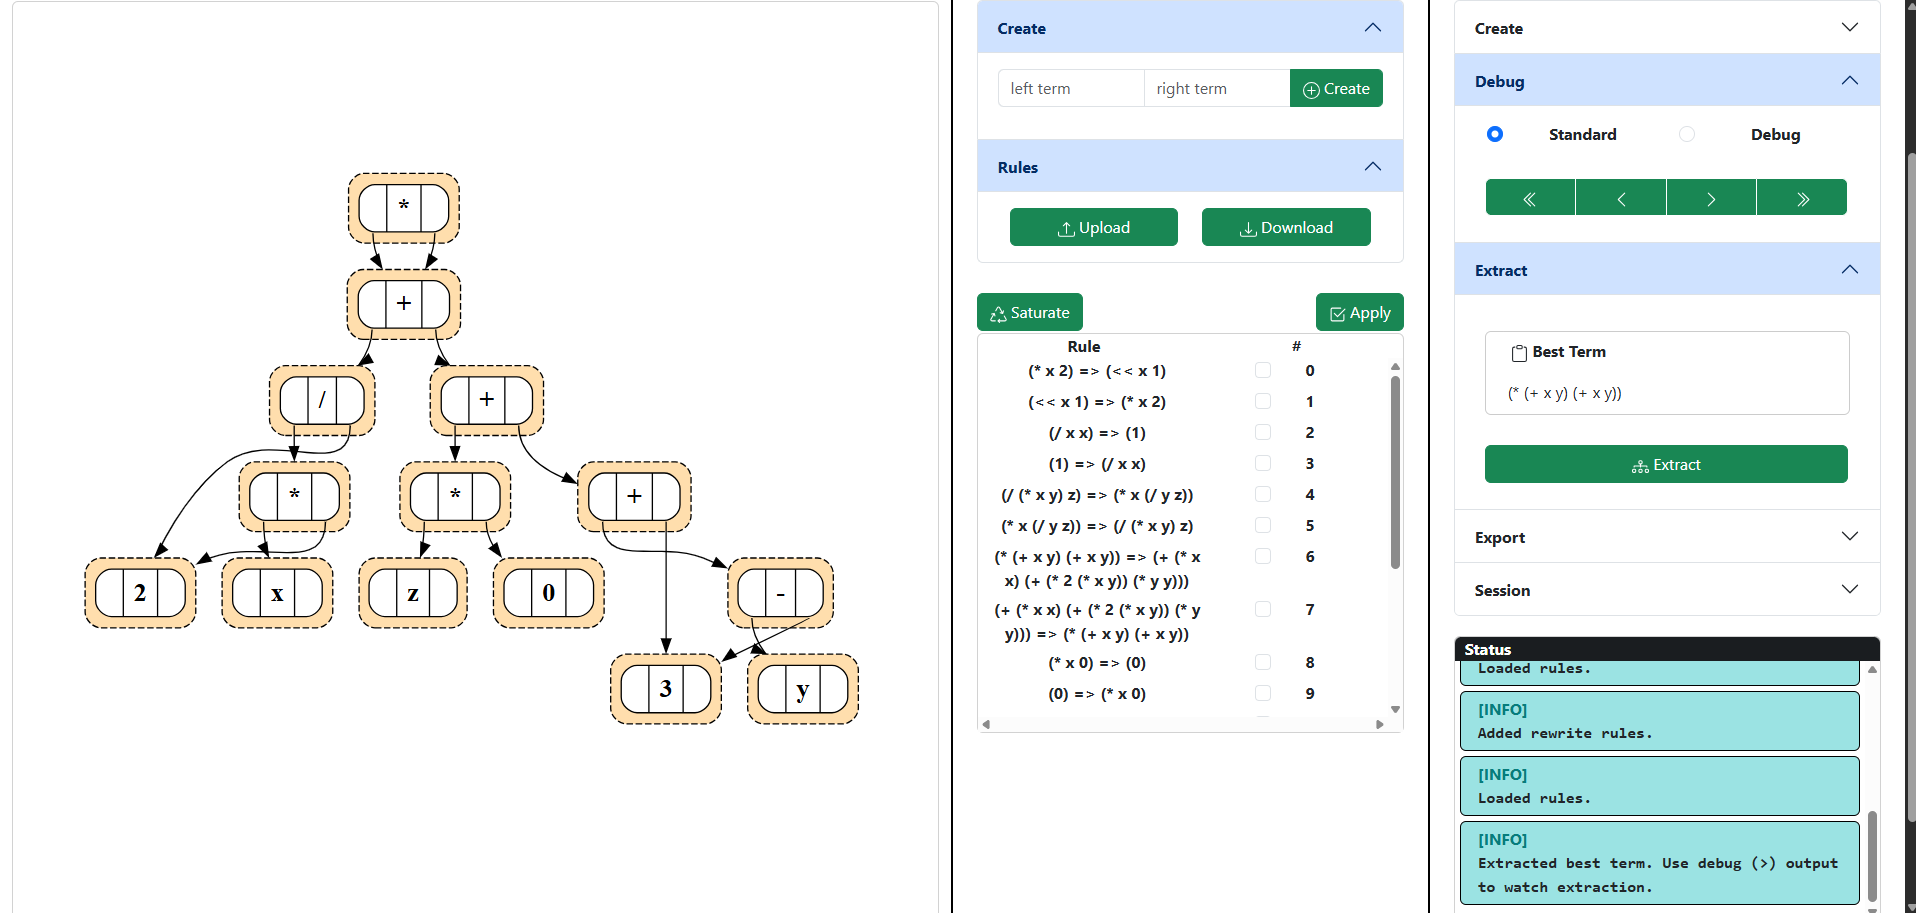
\includegraphics[scale=0.3]{utils/anwendung/anwendung3.png}
    \end{center}
\end{frame}

\begin{frame}{Anwendung (4)}
    \begin{center}
        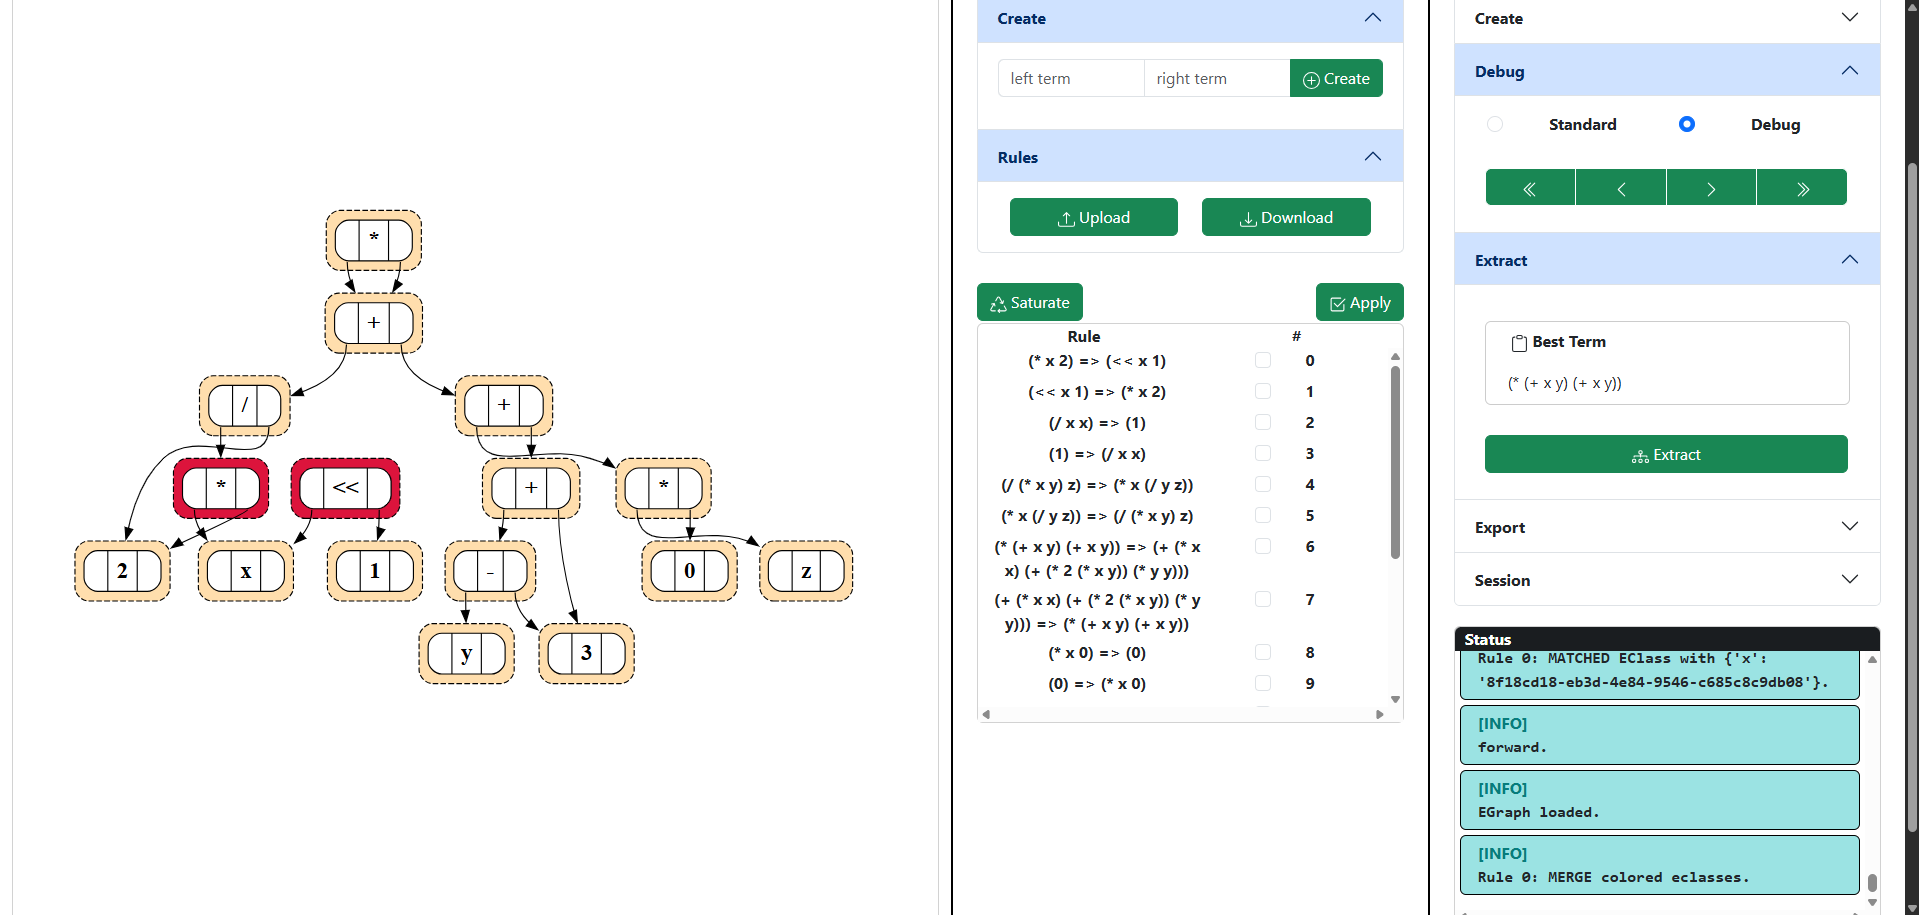
\includegraphics[scale=0.3]{utils/anwendung/anwendung4.png}
    \end{center}
\end{frame}

\begin{frame}{Anwendung (5)}
    \begin{center}
        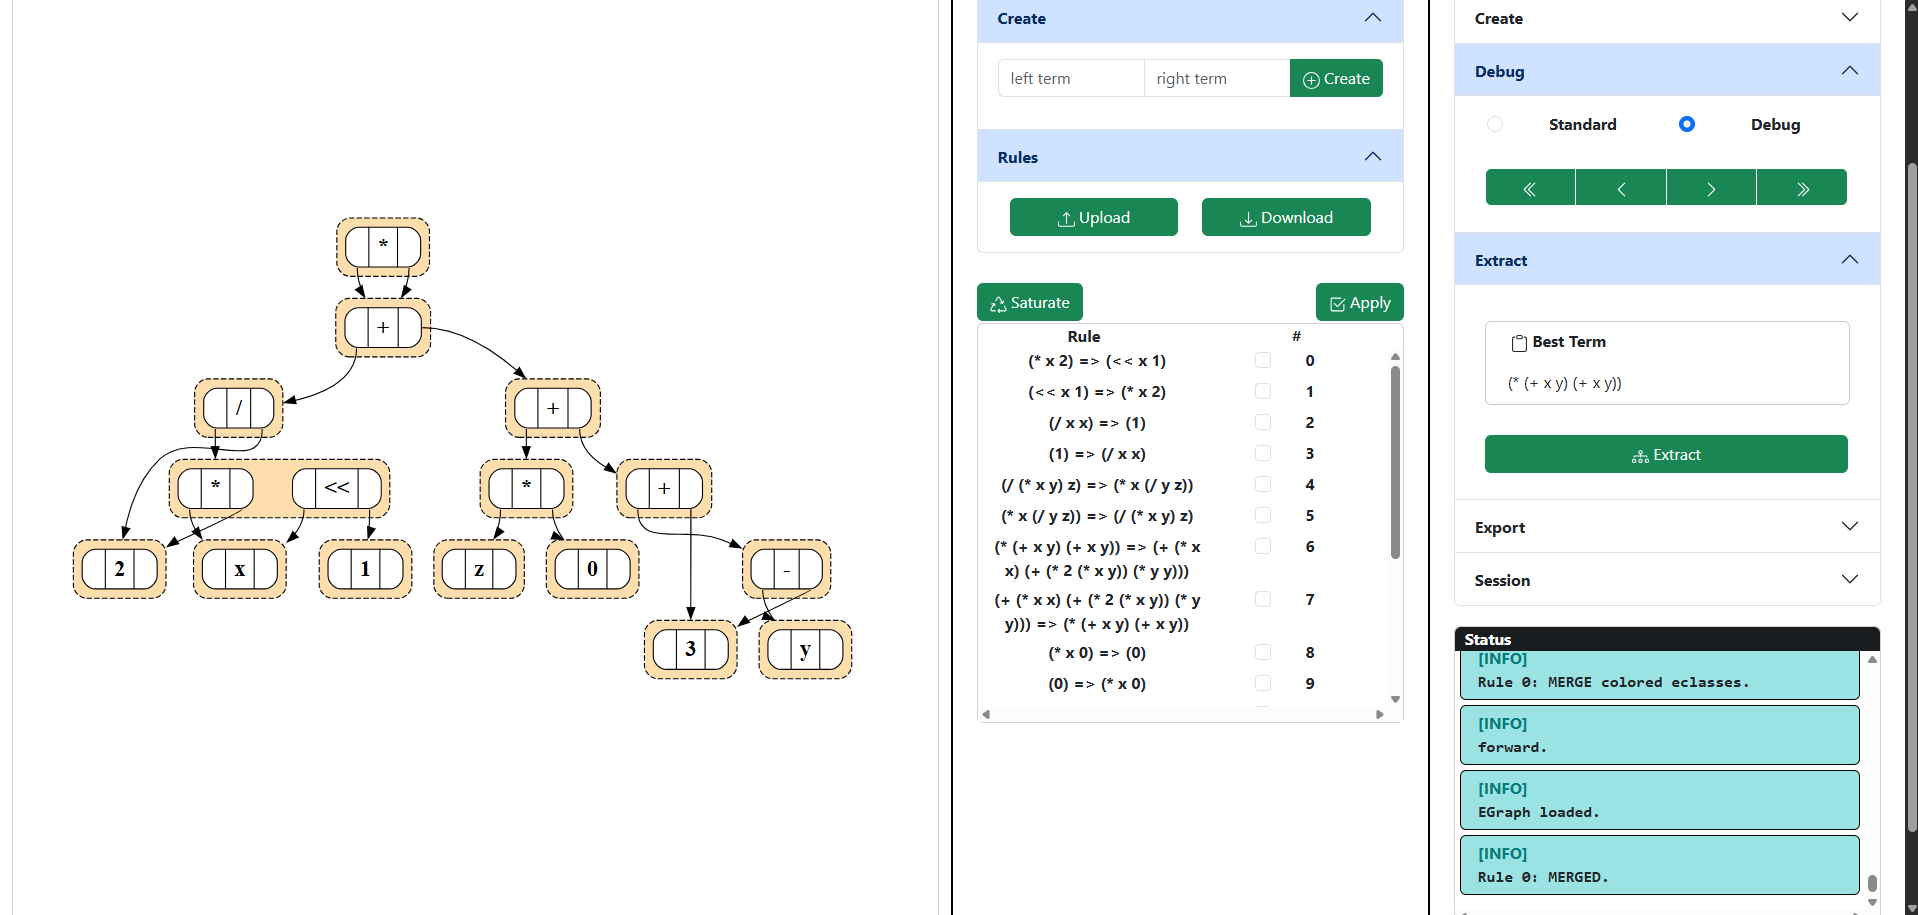
\includegraphics[scale=0.3]{utils/anwendung/anwendung5.png}
    \end{center}
\end{frame}

\begin{frame}{Docs}
    \begin{center}
        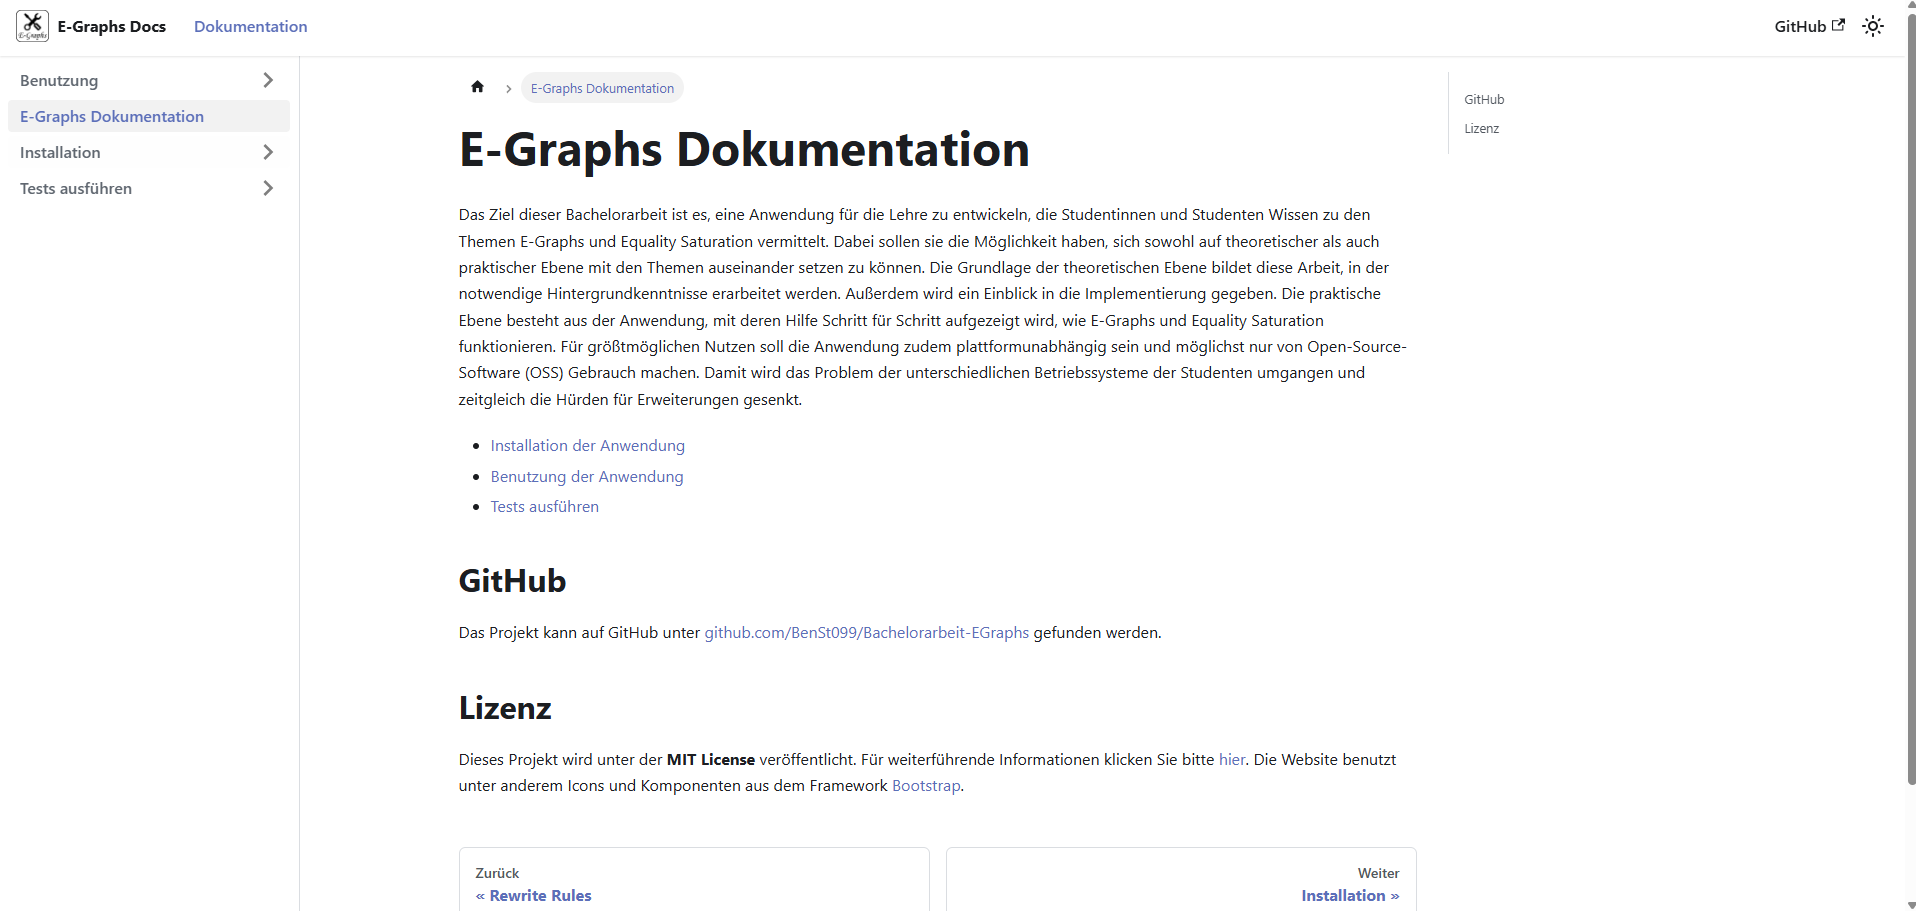
\includegraphics[scale=0.3]{utils/anwendung/docs.png}
    \end{center}
\end{frame}

\begin{frame}{Aufbau}
    \begin{figure}[H]
        \centering
        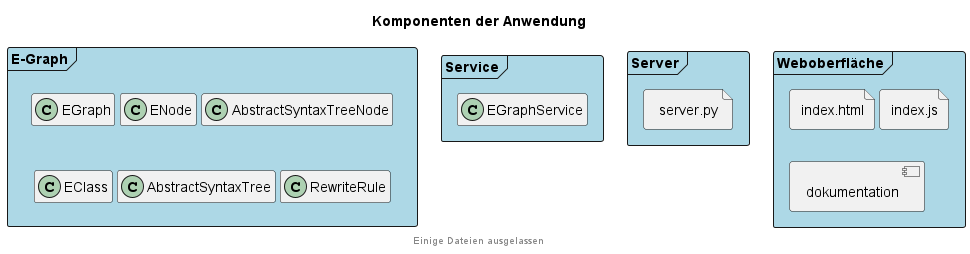
\includegraphics[scale=0.43]{utils/components.png}
        \caption{Architekturdiagramm der Anwendung}
        \label{fig:comps}
    \end{figure}
\end{frame}
